\section{Tipos de servidores}
\label{section:tipos_de_servidores}
Há dois tipos servidores: Servidor de origem e servidor de ponta. Isso independente de suas configurações físicas(quantidade de memória, CPU, HD e \emph{etc}).

\subsection{Servidores de origem}

S\~ao servidores de origem servidores onde toda a informa\c{c}\~ao que irá ser consumida fica baseado. \'E o lugar onde os conte\'udos v\~ao ser primeiramente armazenados e/ou gerados e é o ponto principal do sistema.

\'E ele o respons\'avel por, na aus\^encia da informa\c{c}\~ao perto do cliente, fornecer tudo o que o cliente necessita de informa\c{c}\~ao. Normalmente em primeiros acessos.

H\'a uma necessidade intr\'inseca de que esse servidor tenha excelentes configura\c{c}\~oes f\'isicas e \'otimas regras de seguran\c{c}as, \textit{firewall} a principal delas, que possam garantir a integridade do sistema mesmo em caso de muitos acessos.

\subsection{Servidores de ponta}
S\~ao servidores que mais pr\'oximos aos clientes. Parte do conte\'udo do servidor de origem estar\'a replicado nele. Dizemos em parte, pois n\~ao sabemos quais pol\'iticas de \textit{cache} que ser\'a adotada pelos criadores da rede. 
\\
Podemos ilustr\'a-los conforme a figura \ref{figura:tipos_servidores}.
\begin{figure}[H]
\caption{Tipos de servidores}
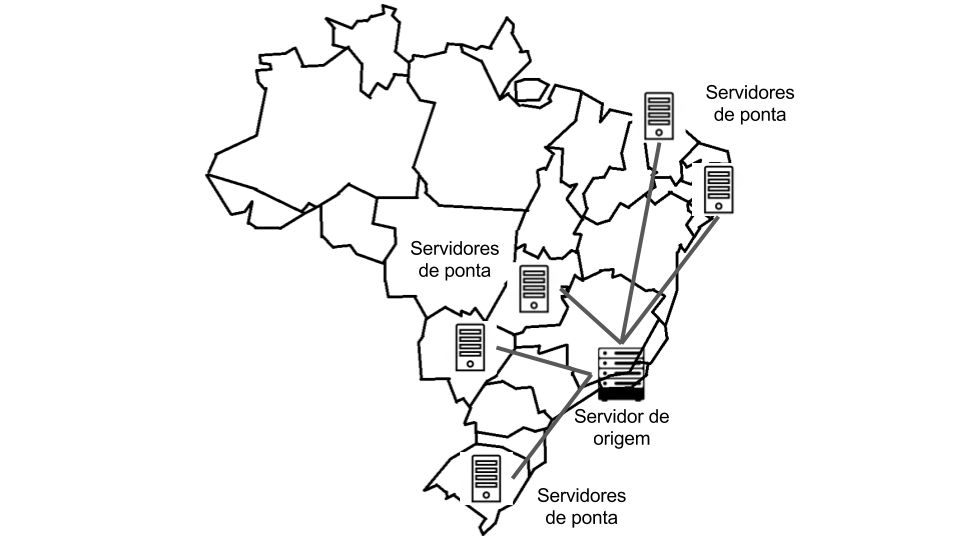
\includegraphics[height=9cm]{Figuras/tipos_servidores.png} 
\label{figura:tipos_servidores} 
\end{figure}

Vale salientar que esses \textit{status} de ser de ponta ou ser de origem não s\~ao imut\'aveis. Em ambientes reais e comerciais um servidor de origem \'e tamb\'em um servidor de ponta para um outro conte\'udo. Isso \'e o respons\'avel por tornar as grandes \emph{CDNs} completamente transparentes geograficamente perante aos seus clientes.